\documentclass{beamer}
\usepackage[T1]{fontenc}
\usepackage[utf8]{inputenc}
\usepackage{lmodern}
\usepackage[francais]{babel}
\usepackage{graphicx}
\usepackage{ulem}
\usepackage{pgfpages}
\usepackage{pgfplots}
\graphicspath{{./fig/}}
\usetheme[]{ens}


%\usetheme[sectiontitle]{crans}
\title{Le traitement du signal \\et le post-bac}
% A subtitle is optional and this may be deleted
\subtitle{}
\author[]{\textsc{Pierre-Antoine Comby}}
\institute{pierre-antoine.comby@ens-paris-saclay.fr}
\date{\today}
\setbeameroption{show notes on second screen}
\tikzset{every picture/.style={execute at begin picture={\shorthandoff{:;!?};}}}

\pgfplotsset{
  timeplot/.style={
    xlabel={\tiny$t[s]$},ylabel={\tiny$x(t)$},
    axis lines=middle,
    xlabel style={at=(current axis.right of origin), anchor=west},
    ylabel style={at=(current axis.above origin), anchor=south},
    ticks=none,
    enlarge y limits={rel=0.13},
    enlarge x limits={rel=0.07},
  },
  freqplot/.style={
    xlabel={\tiny$f[Hz]$},ylabel={\tiny$A(f)$},
    axis lines=middle,
    xlabel style={at=(current axis.right of origin), anchor=west},
    ylabel style={at=(current axis.above origin), anchor=south},
 %   enlarge y limits={rel=0.13},
    enlarge x limits={rel=0.07},
    ticks=none,
  }
}


\begin{document}
\begin{frame}
   \titlepage
\end{frame}

% \begin{frame}{Sommaire}
%   \tableofcontents[subsubsectionstyle=hide]
% \end{frame}
\begin{frame}{Objectif de la séance}
  \begin{itemize}
    \item Donner un avant goût des études supérieures en maths/physique.
    \note[item]{ Exemple de la ``voie royale''/parcours d'excellence. Ne pas négliger les parcours universitaires, plus spécifiques.}
    \item Introduire des notions niveau bac/bac+1 de traitement du signal (utile pour un TPE par ex.)
    \note[item]{Avec le moins de prérequis possible, pas facile, il va falloir rester bien concentré. Ne pas hésiter à lever la main. Donner votre Prénom}
    \item Présenter mon parcours et mon travail actuel.
  \end{itemize}
\end{frame}

\section{Mon parcours}
\label{sec:label}
\begin{frame}{Curriculum Vitae}
  \begin{description}
    \item[2012-2015:] Lycée Charles Péguy, BAC S , ABIBAC.
    \item[2015-2017:] Classe Prépa (Lycée Saint Louis, Paris)
      \begin{itemize}
        \item PCSI
        \item PSI*
      \end{itemize}
    \item[2017-2021:] Ecole Normale Supérieure \sout{Cachan} Paris-Saclay
      \begin{itemize}
        \item L3 Sciences de l'ingénieur/Physique
        \item M1 Electronique, Electrotechnique, Automatique
        \item \textit{M2 Stage de recherche à Karlsruhe: Tomographie à ultrason, imagerie médicale}
        \item \textcolor{gray}{M2R: Master Traitement du Signal/IA}
      \end{itemize}
    \item[2021-futur:] \textcolor{gray}{Probablemement une thèse}.
  \end{description}
\end{frame}
\note{Un peu de chance, un peu de talent, beaucoup de travail}

\section{Introduction au traitement du signal}
\subsection{Définition}
\label{sec:label}
\begin{frame}{Le traitement du signal}
  \begin{block}{Définition}
    \begin{itemize}
      \item Un \textbf{signal} est une fonction d'une ou plusieurs variables qui véhicule de l'information sur un phénomène physique.
      \pause
      \item Un \textbf{système} (de traitement du signal) transforme un ou des signaux en d'autres signaux ou paramètre, dans le but d'en extraire de l'information.
      \end{itemize}
  \end{block}
  \begin{exampleblock}{Application}
    \begin{columns}
      \begin{column}{0.5\textwidth}
        \begin{itemize}
          \item mesures physiques
          \item télécommunication
          \item Fusées
          \item Musique
        \end{itemize}
      \end{column}\pause
      \begin{column}{0.5\textwidth}
        \begin{itemize}
          \item Traitement d'image
          \item Biologie
          \item Imagerie médicale,
          \item mécanique, etc
        \end{itemize}
      \end{column}
    \end{columns}
  \end{exampleblock}
\end{frame}
\begin{frame}{Exemple élémentaire de TS}
  \setlength{\leftmargini}{2.5cm}         %new code: set margin length to 0
  \begin{itemize}
    \item[Mesure:\pause] Estimation de grandeurs caractéristiques\pause
    \note[item]{grandeurs statistiques}
    \item[Détection:\pause] Extraction d'un signal utile du bruit\pause
    \note[item]{temps d'arrivée d'un signal}
    \item[Filtrage:\pause] Élimination de composante indésirable\pause
    \note[item]{Oreilles, séparer basse et aigus, retirer le bruit, Instagram}
    \item[Codage:\pause] Mise en forme pour transmission\pause
    \note[item]{Toutes les communications numériques}
    \item[Compression:\pause] Réduction de la redondance d'information.\pause
    \note[item]{JPEG(3 à 100 fois plus petit), MP3, faire une fiche de cours}
    \item[Modulation:\pause] Adaptation d'un signal aux caractéristiques d'une voie de transmission\pause
    \note[item]{radio AM (WW2), FM }
    \item[Segmentation:\pause] Découpage en parties homogènes\pause
    \note[item]{Imagerie médicale, Filtre snapchat}
    \item[Reconnaissance:\pause] Identification de formes appartenant à un dictionnaire.\pause
    \note[item]{Filtre Snapchat}
  \end{itemize}
\end{frame}

\begin{frame}{Encore des exemples}
  \centering
  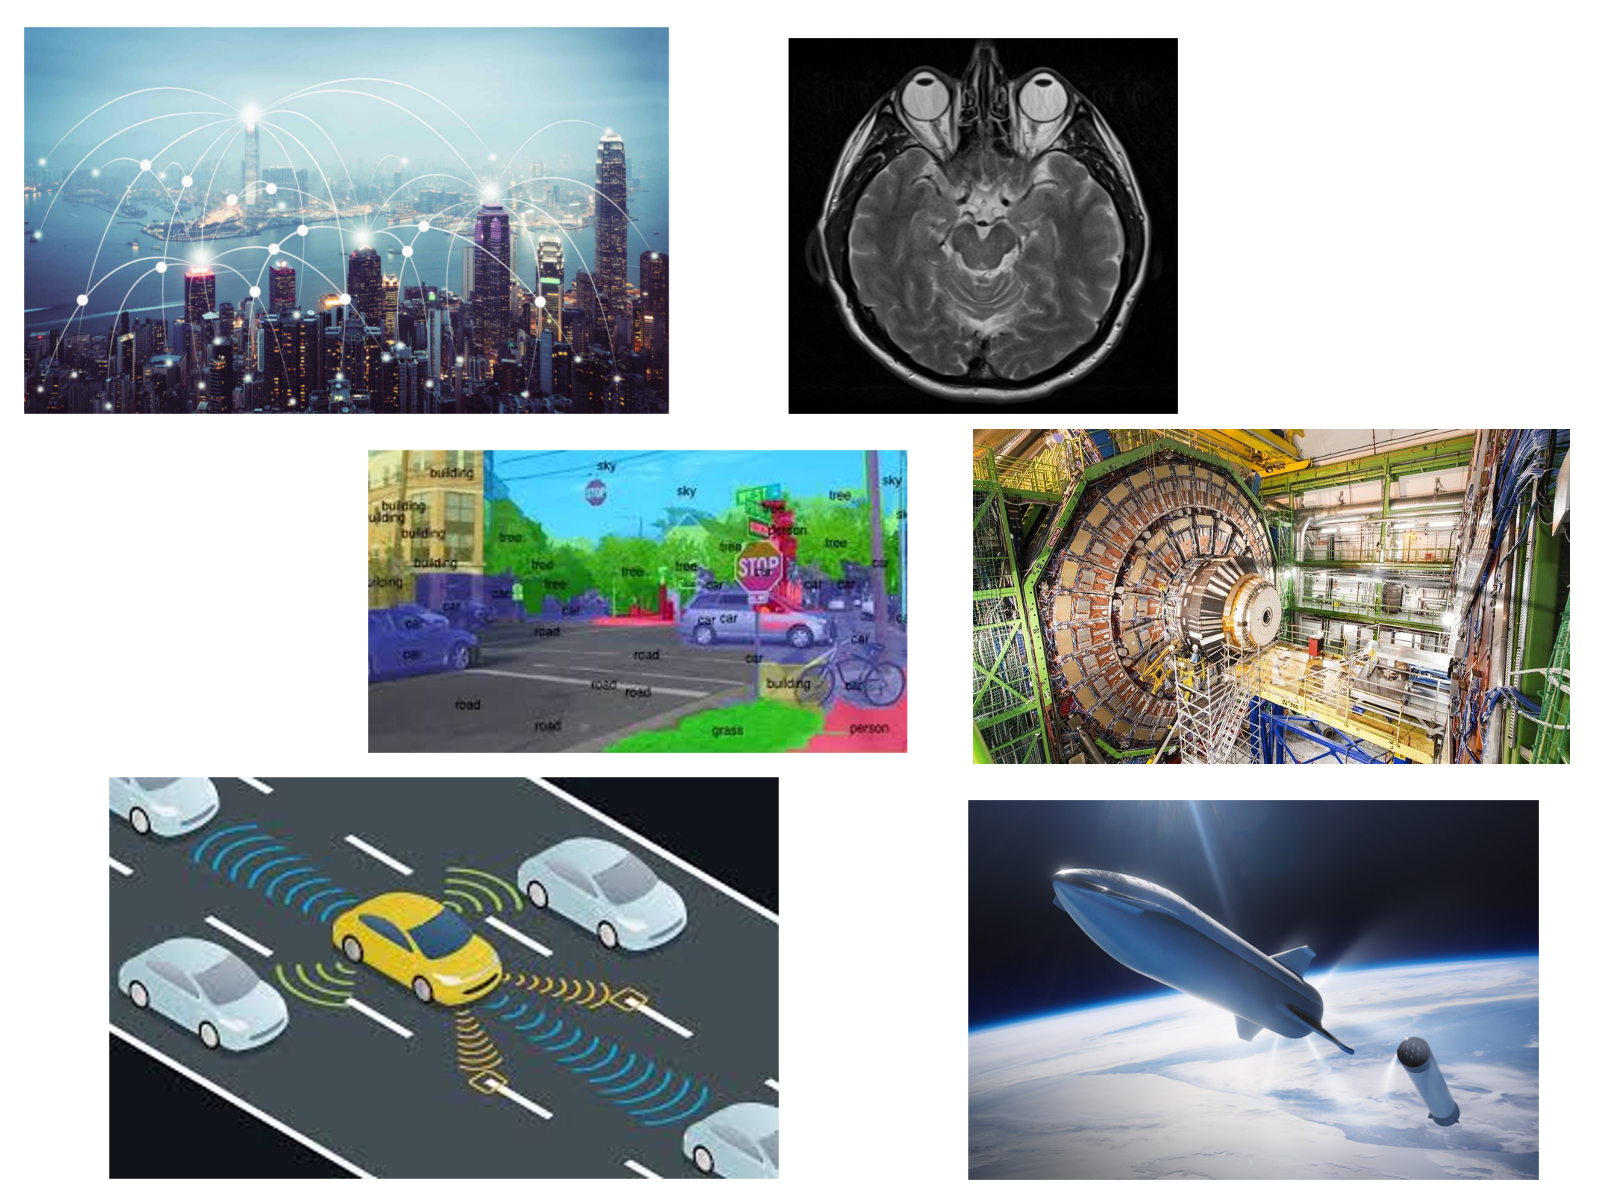
\includegraphics[width=\textwidth]{buzz.png}
\end{frame}
\note[enumerate]{
  \item Smart City: 5G, transmission, compression, analyse,
  \item IRM de cerveau -> imagerie médicale: filtrage, segmentation, reconstruction/synthèse\ldots
  \item Vision Artificielle: segmentation, reconnaissance, fiabilité
  \item LHC: les tres grands instruments pour voir le tout petit
  \item Voiture Autonome: protocoles de transmission, sécurité
  \item SpaceX -> aérospatial: communiquer sur des miliers de kilomètre: modulation, codage, compression
}
\begin{frame}{Classification des signaux}
  \begin{itemize}
    \item Nombre de variable (1-D (son), 2-D (image), N-D,\ldots)
    \item réel/complexe
    \item périodiques (ex: $\cos(2\pi ft)$)
    \item Déterministe/aléatoire
    \begin{itemize}
      \item déterministe: évolution complètement prédictible
      \item aléatoire: non prédictible, non reproductible.
    \end{itemize}
    \item Continus / Discret
    \begin{itemize}
      \item Analogique/Numérique
    \end{itemize}
  \end{itemize}
\end{frame}
\subsection{Dualité Fréquentielle}
\begin{frame}[fragile]{Analyse Spectrale}
  \vspace*{-1em}
  \begin{block}{Expérience}
    \begin{itemize}
      \item<1-> 3 sons à la même fréquence, mais différente forme d'onde.
      \item<5-> On entend d'autres fréquences, sans les voir: \visible<5->{\it un spectre}
    \end{itemize}

  \end{block}
  %% Time
  \begin{columns}
    \begin{column}{0.3\textwidth}
      \centering
      \begin{tikzpicture}
        \begin{axis}
          [width=1.33\textwidth, height=0.4\textheight,
          domain =0:10,
          timeplot]
          \addplot+[no marks, smooth]{sin(360*x/5)};
        \end{axis}
      \end{tikzpicture}\pause[3]
    \end{column}
    \begin{column}{0.3\textwidth}
      \centering
      \begin{tikzpicture}
        \begin{axis}
          [timeplot, width=1.33\textwidth, height=0.4\textheight,]
          \addplot+[mark=none] coordinates {
            (0,0) (1.25,1) (3.75,-1) (6.25,1) (8.75,-1) (10,0)
          };
        \end{axis}
      \end{tikzpicture}\pause[4]
    \end{column}
    \begin{column}{0.3\textwidth}
      \centering
      \begin{tikzpicture}
        \begin{axis}
          [timeplot,
          width=1.33\textwidth, height=0.4\textheight,]
          \addplot+[mark=none,const plot] coordinates {
            (0,1) (2.5,-1) (5,1) (7.5,-1) (10,1)
          };
        \end{axis}
      \end{tikzpicture}\pause[4]
    \end{column}
  \end{columns}
  %% Freq
  \note{La3: 440 Hz,  apporter ordi/téléphone + Enceinte}
  \pause[6]
  \begin{columns}
    \begin{column}{.3\textwidth}
       \begin{tikzpicture}
        \begin{axis}
          [freqplot,
          width=1.33\textwidth, height=0.4\textheight, ticks=none,
          xmin=0,xmax=10,ymin=0,ymax=1.2,
          ]
          \draw[blue]
          (axis cs:1,0) -- (axis cs:1,1)   node{$\cdot$};
        \end{axis}
      \end{tikzpicture}
    \end{column}
    \begin{column}{.3\textwidth}
       \begin{tikzpicture}
        \begin{axis}
          [freqplot,width=1.33\textwidth, height=0.4\textheight,
          xmin=0,xmax=10,ymin=0,ymax=1.2,
          ]
          \draw[blue]
          (axis cs:1,0) -- (axis cs:1,1)    node{$\cdot$}
          (axis cs:3,0) -- (axis cs:3,0.11) node{$\cdot$}
          (axis cs:5,0) -- (axis cs:5,0.04) node{$\cdot$}
          (axis cs:7,0) -- (axis cs:7,0.02) node{$\cdot$}
          (axis cs:9,0) -- (axis cs:9,0.012)node{$\cdot$}
          ;
        \end{axis}
      \end{tikzpicture}
    \end{column}
    \begin{column}{.3\textwidth}
       \begin{tikzpicture}
        \begin{axis}
          [freqplot, width=1.33\textwidth, height=0.4\textheight,
          xmin=0,xmax=10,ymin=0,ymax=1.2,
          ]
          \draw[blue]
          (axis cs:1,0) -- (axis cs:1,1)    node{$\cdot$}
          (axis cs:3,0) -- (axis cs:3,0.33) node{$\cdot$}
          (axis cs:5,0) -- (axis cs:5,0.2)  node{$\cdot$}
          (axis cs:7,0) -- (axis cs:7,0.143)node{$\cdot$}
          (axis cs:9,0) -- (axis cs:9,0.111)node{$\cdot$}
          ;
      \end{axis}
    \end{tikzpicture}
  \end{column}
 \end{columns}
\end{frame}

\note{%
  Joseph Fourier, 1806, préfet de l'Isère. Travail sur l'équation de la chaleur (anneau en métal chauffé)

}%
\begin{frame}{Décomposition de Fourier}
  \framesubtitle{Les maths}
  \begin{alertblock}{Théorème (Lycée)}
    Toute fonction périodique peux s'écrire comme une somme pondérée de fonction sinusoïdale
    \[
      x_{per}(t) = \sum_{n=0}^{+\infty}a_{n}cos(2\pi n f_{0}t)+b_{n}sin(2\pi n f_{0}t)
    \]
  \end{alertblock}
  \begin{itemize}
    \item $(a_{n})$ et $(b_{n})$ sont des suites, appelées coefficients de fourier.
    \item Les coeffients s'obtienne par produit scalaire sur des fonctions.
      \note[item]{$a_{n} = \int_{-T/2}^{T/2}x(t)\cos(2\pi nft)dt$}
    \item Théorème généralisable a toute fonction à énergie fine ($\sim$ toutes les fonctions en physiques).
      \note[item]{$X(f)=\int_{-\infty}^{+\infty}x(t)e^{-2\pi i ft}d t$}
  \end{itemize}

\end{frame}
\begin{frame}[fragile]{Décomposition de Fourier}
  \framesubtitle{La physique}
  \begin{tikzpicture}
    \begin{axis}[timeplot,domain=0:10,
      height=0.6\textheight,width=1.1\textwidth]
      \visible<1->{
      \addplot[mark=none,const plot] coordinates {
        (0,1) (2.5,-1) (5,1) (7.5,-1) (10,1)
      };}
      \foreach \i [count=\ii] in {1,3,5,15,50}{
        \only<+(1)>{
          \addplot+[mark=none,blue] table [x=x, y=\i, col sep=comma] {creneau.csv};}
      }
    \end{axis}
  \end{tikzpicture}\\
  \begin{tikzpicture}
\begin{axis}
          [freqplot, width=\textwidth, height=0.3\textheight,
          xmin=0,xmax=15,ymin=0,ymax=1.2,
          ]
          \draw<2->[blue](axis cs:1,0) -- (axis cs:1,1)    node{$\cdot$};
          \draw<3->[blue](axis cs:3,0) -- (axis cs:3,0.33) node{$\cdot$};
          \draw<4->[blue](axis cs:5,0) -- (axis cs:5,0.2)  node{$\cdot$};
          \draw<5->[blue]
          \foreach \x in {7,9,...,15}{
            (axis cs:\x,0) -- (axis cs:\x,1/\x)  node{$\cdot$}
          };
      \end{axis}
  \end{tikzpicture}
      $\hat{x}(t)=
      \visible<2->{\frac{4A}{\pi}\times\left[\sin(2\pi f_{0}t)\right.}
      \visible<3->{+\frac{1}{3}\sin(2\pi 3f_{0}t)}
      \visible<4->{+\frac{1}{5}\sin(2\pi 5f_{0}t)}
      \visible<5->{+\cdots}
      \visible<2->{\left.\right]}$
\end{frame}
\note{phénomène de Gibbs, du a la discontinuité de la fonction créneau}
\begin{frame}{Dualité temps-fréquence}
  \begin{alertblock}{À retenir}
    Tout signal ``physique'' possède un unique signal équivalent dans le domaine \emph{fréquentiel}. L'operation pour passer de l'un à l'autre est appelé \emph{transformée de Fourier}
  \end{alertblock}
  \begin{itemize}[<+->]
    \item Preuve : Bac+3, rigoureux en Bac+5
    \item \emph{Tout} type de signaux (son,image, volume 3D)
    \note[item]{la ou il y a du signal, il y a une TF}
  \end{itemize}\pause
  La transformée de fourier est utilisé notamment en:
  \begin{itemize}[<+->]
    \item physique quantique
    \item compression d'image
    \item cryptographie
    \item ...
  \end{itemize}


\end{frame}

\subsection{Conversion Analogique Numérique}
\begin{frame}{Analogique vs Numérique}
  \framesubtitle{Exemples}
      \note{Demander 3 exemples Analogique, Numériques}
  \begin{columns}
    \begin{column}{.5\textwidth}
      Signaux Analogiques:\pause[1]
      \begin{itemize}
        \item la voix,
        \item piste vinyle
        \item les rayons du soleil
        \item L'altitude
      \end{itemize}
      \pause[2]
      \begin{block}<4>{}
        \begin{itemize}
          \item Continus
          \item Valeurs quelconques
        \end{itemize}
      \end{block}
    \end{column}
    \begin{column}{.5\textwidth}
      Signaux Numériques:\pause[3]
      \begin{itemize}
        \item piste CD
        \item Images
        \item métronome
        \item 100111101
      \end{itemize}
      \begin{block}<4>{}
        \begin{itemize}
          \item temps discret
          \item valeurs limitées
        \end{itemize}
      \end{block}
    \end{column}
  \end{columns}
\end{frame}

\begin{frame}{Conversion Analogique Numérique}
  \framesubtitle{Généralité}
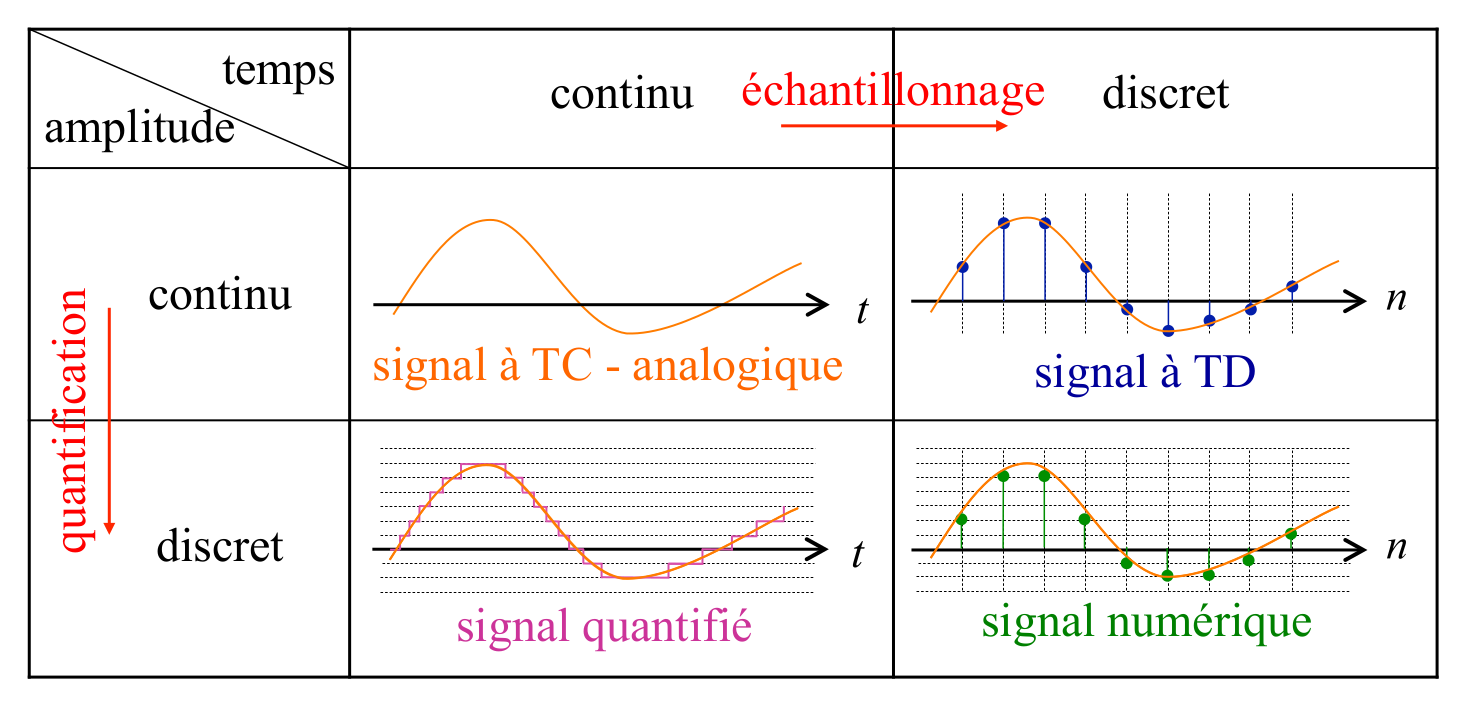
\includegraphics[width=\textwidth]{fig/discret-continu}
\end{frame}
\begin{frame}{Echantillonage}

\end{frame}
\begin{frame}{Quantification}

\end{frame}




\section{Vos Question}

\begin{frame}
\begin{tikzpicture}[remember picture,overlay]
\fill[bleuens](current page.north west) rectangle (current page.south east);
\node at ([yshift=+.15\textheight]current page.center) (title)
  {\usebeamerfont{title}\textcolor{white}{Merci pour votre attention}};

\node[below=2em]
  at(title) (subtitle)
  {\usebeamerfont{subtitle}\textcolor{white}{Des questions ?}};

\node
  at ([yshift=-70pt]current page.center) (institute)
  {\usebeamerfont{institute}\textcolor{white}{\insertinstitute}};

\node
  at ([yshift=-50pt]current page.center) (author)
  {\usebeamerfont{author}\textcolor{white}{\insertauthor}};

\node[anchor=north west]
  at (current page.north west) (logo)
  {\usebeamercolor[fg]{titlegraphic}
    
\includegraphics[scale=0.3]{ENSPS-revert.png}};
\end{tikzpicture}
\end{frame}
\note{Demander les noms, 1/2 1/2 1/2
  \item La prépa/L'ENS/Le supérieur
  \item Le TS
  \item Bonus: la recherche, au tableau
}
\end{document}

%%% Local Variables:
%%% mode: latex
%%% TeX-master: t
%%% ispell-local-dictionary: "francais"
%%% End:
